\section{Network testing}
\textbf{Выданные параметры:} [netdev,netlink-task]
\subsection{netlink-task}
\nquote{--netlink-task N}{start  N workers that collect task statistics via the netlink taskstats interface.  This stressor can
only be run on Linux and requires CAP\_NET\_ADMIN capability.}
\nquote{netlink}{это специальное семейство адресов сокетов (AF\_NETLINK), предназначенных для получения информации о ядре. Процедура использования netlink включает открытие сетевого сокета с семейством адресов AF\_NETLINK и последующее выполнение серии вызовов send(2) и recv(2) для передачи запросов и получения информации в двоичных структурах.}
Найдем оптимальное количество воркеров:\\
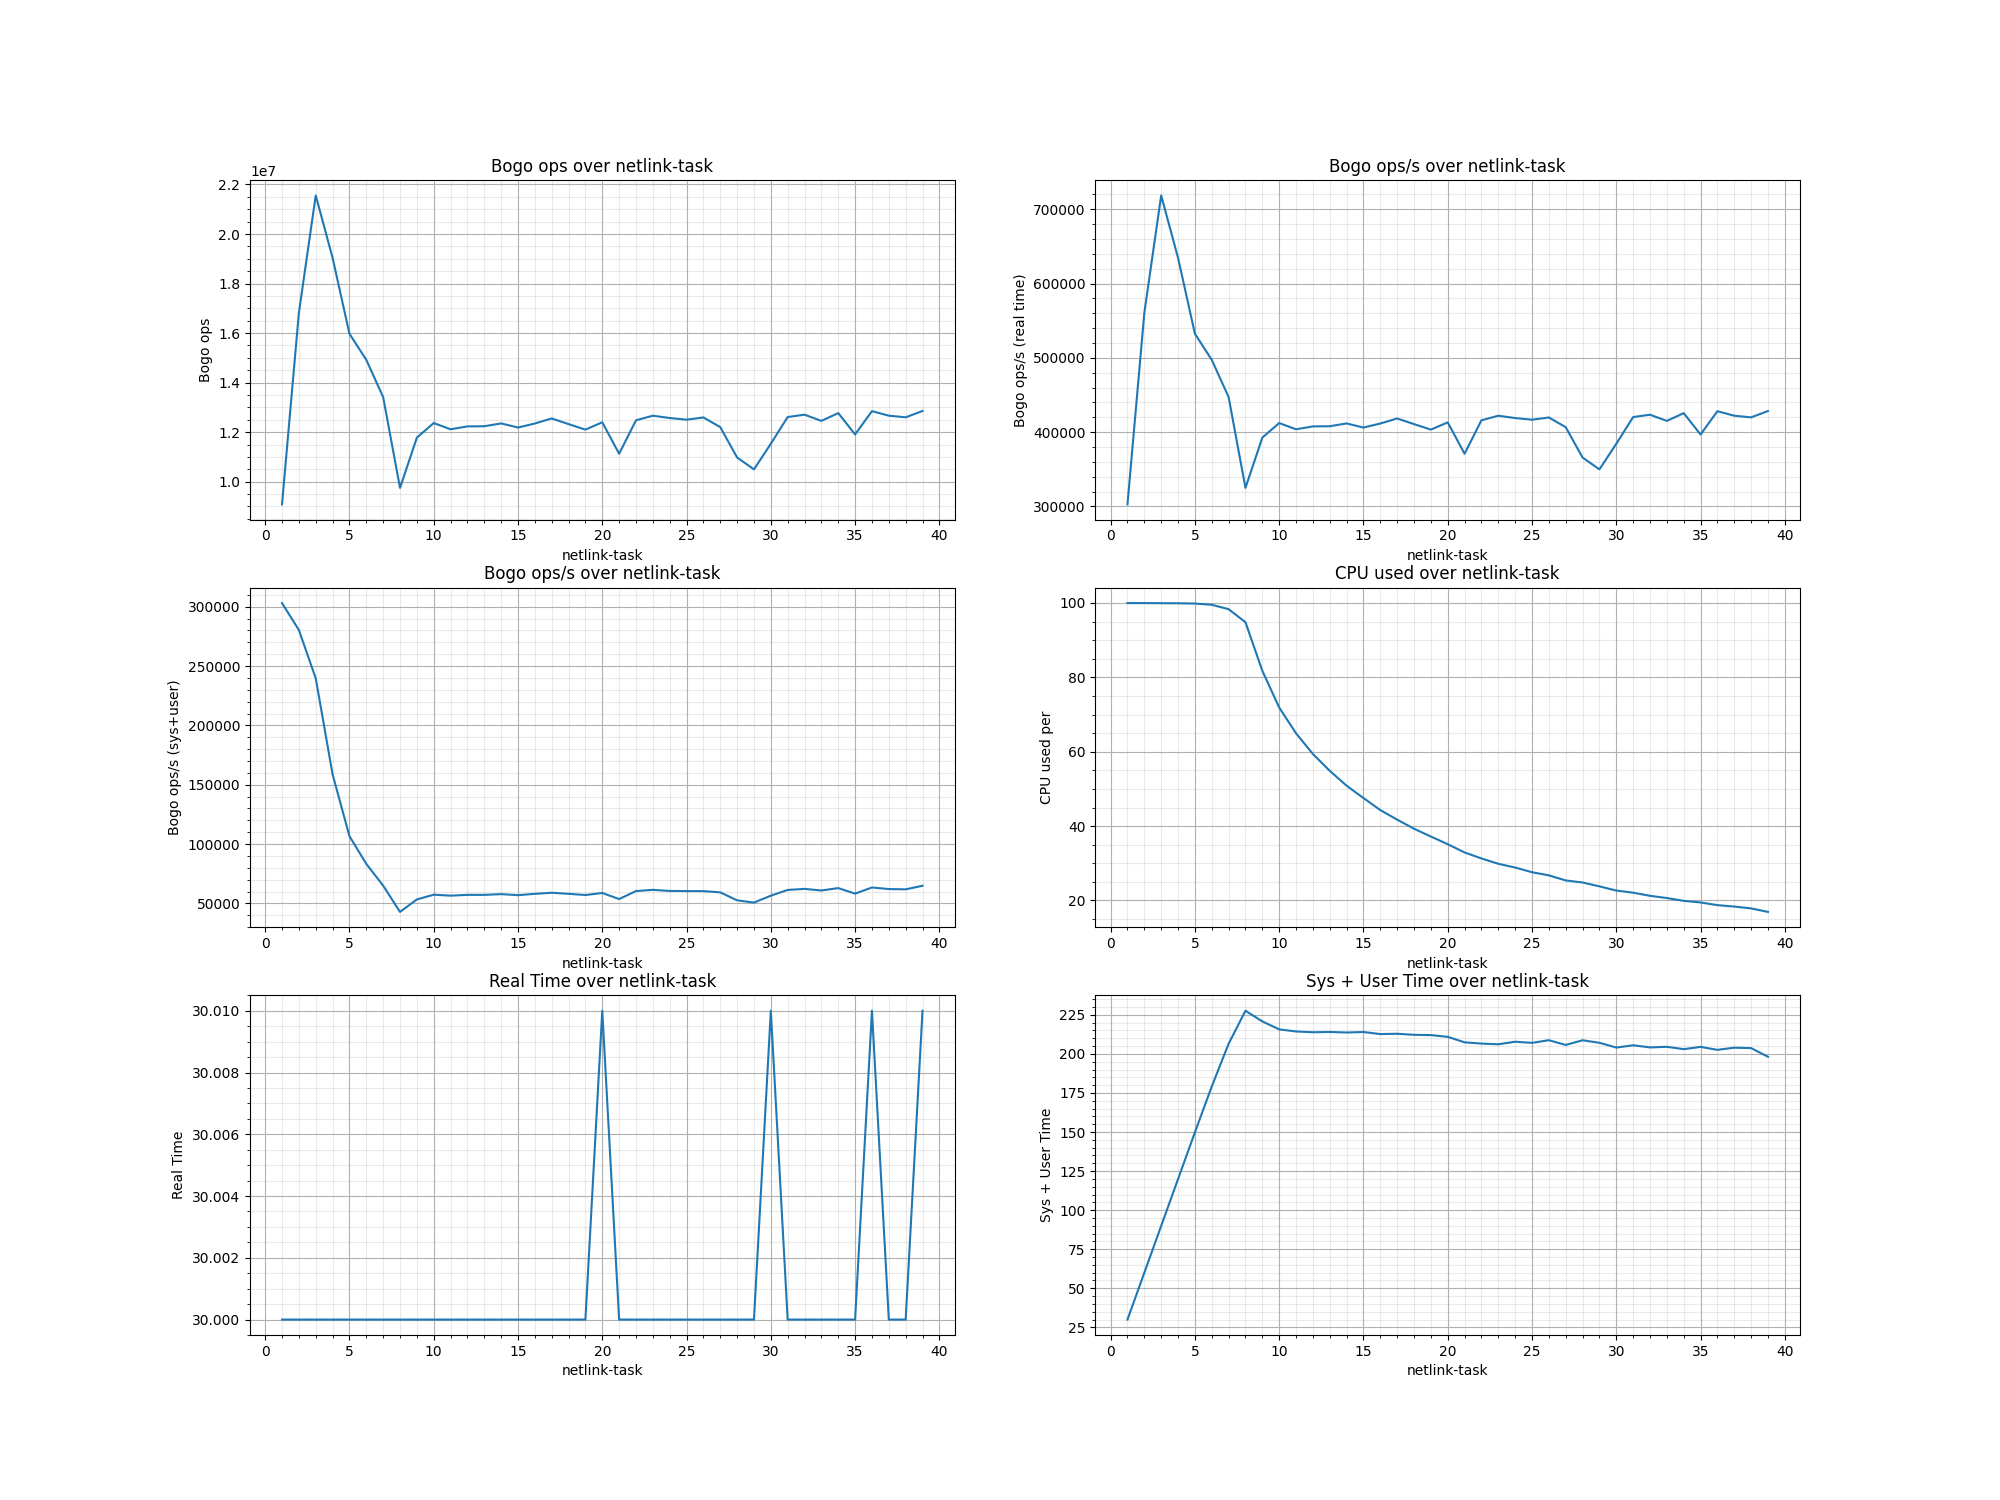
\includegraphics[width=\textwidth]{./network/image/netlink-task-bogops.png}
Максимум bogo ops достигается при 3.
С помощью команды \textit{ss -a} мы можем посмотреть с какими сокетами работает stress-ng:\\
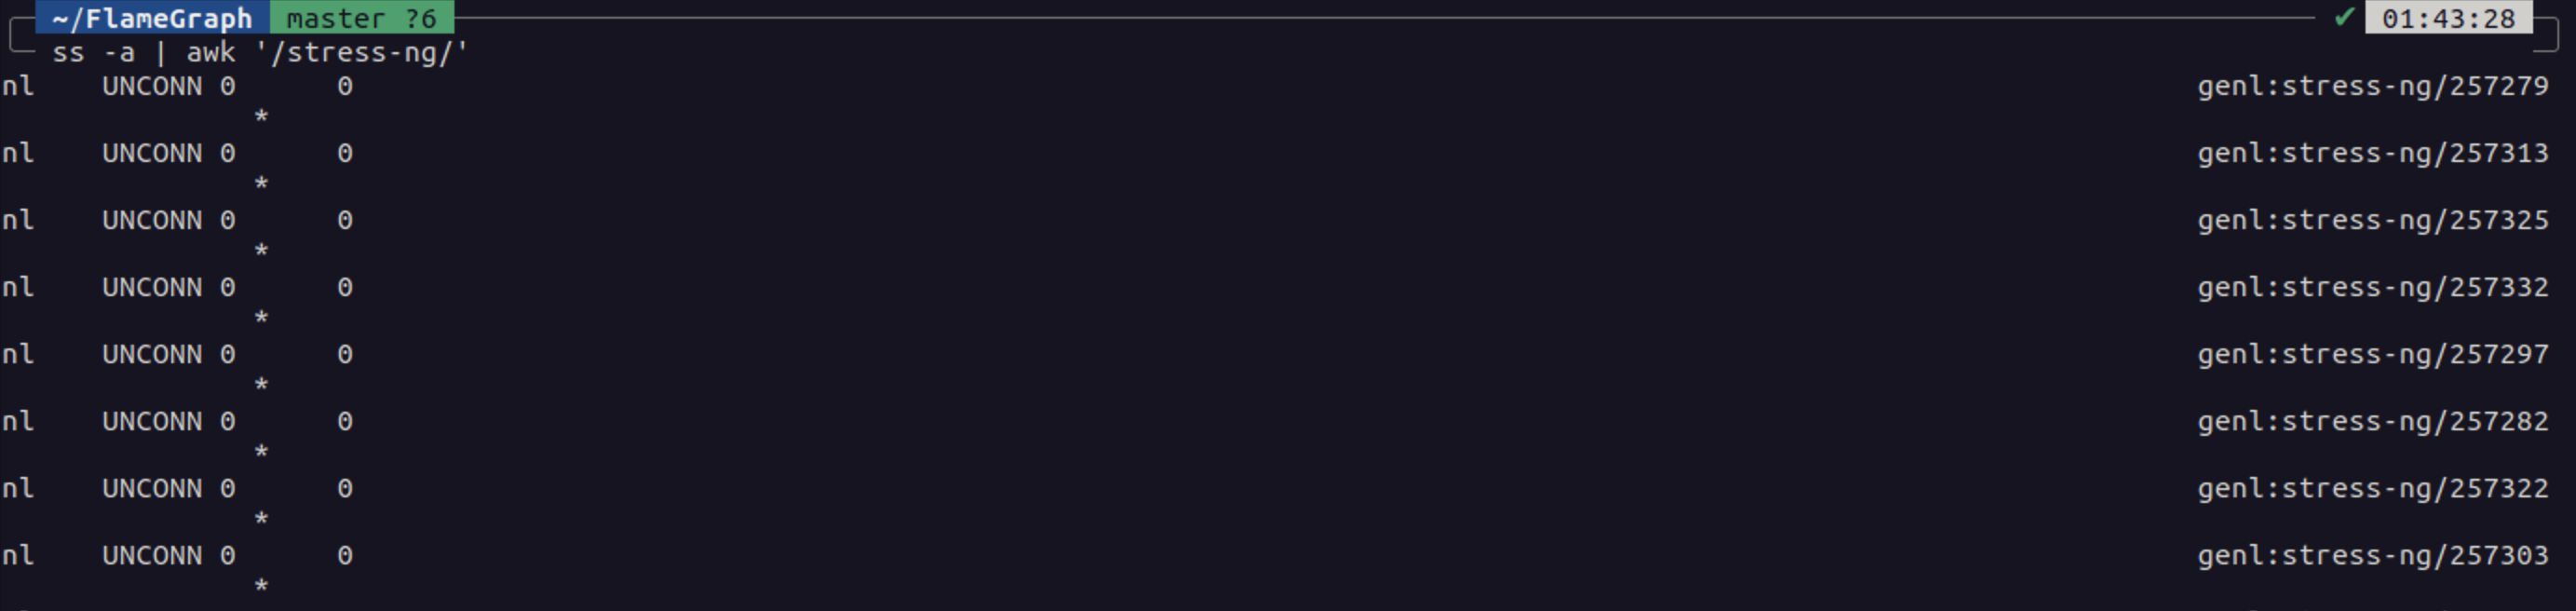
\includegraphics[width=\textwidth]{./network/image/netlink-ss.png}
Также нагрузку, которую создает \textit{netlink-task} на \textit{netlink} можно заметить если запустить параллельно другой тест работающий с \textit{netlink}.
\nquote{--netlink-proc N}{start N workers that spawn child processes and monitor fork/exec/exit process events via the proc netlink connector. Each event received
is counted as a bogo op. This stressor can only be run on Linux and requires CAP\_NET\_ADMIN capability.}
Напишим скрипт запускающий несколько раз netlink-proc с netlink-task и без, сравним bogo ops.\\
\lstinputlisting[]{network/scripts/netlink-proc.zsh}
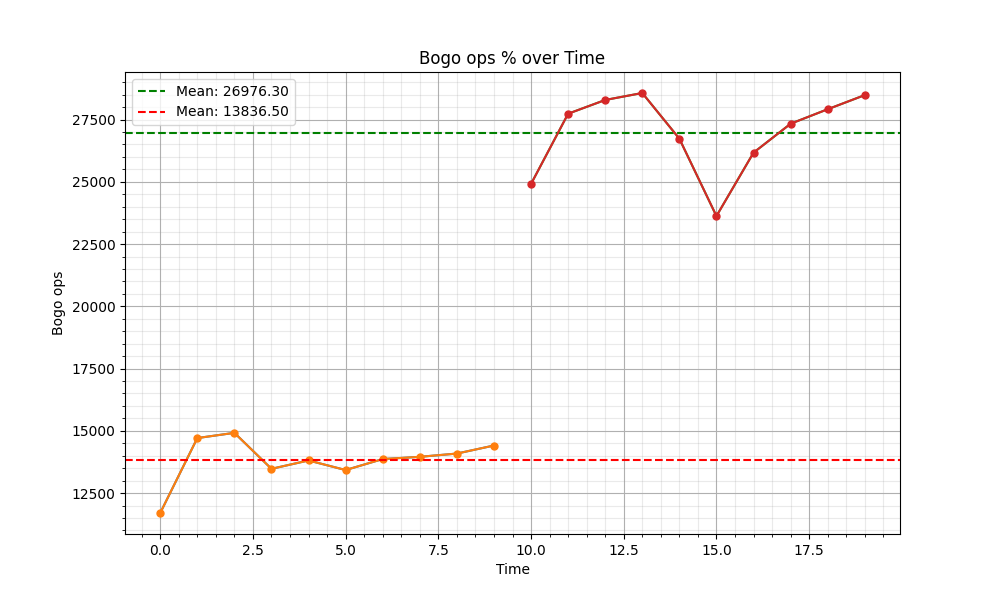
\includegraphics[width=\textwidth]{./network/image/netlink-proc.png}
Видим, что из-за нагрузки производительность netlink падает.\\


\subsection{netdev}
\nquote{--netdev N}{start N workers that exercise various netdevice ioctl commands across all the available  network  devices.  The ioctls exercised by this stressor are as follows: SIOCGIFCONF, SIOCGIFINDEX, SIOCGIFNAME,
SIOCGIFFLAGS, SIOCGIFADDR, SIOCGIFNETMASK, SIOCGIFMETRIC, SIOCGIFMTU, SIOCGIFHWADDR,  SIOCGIFMAP  and
SIOCGIFTXQLEN. See netdevice(7) for more details of these ioctl commands.}
Найдем оптимальное количество воркеров:\\
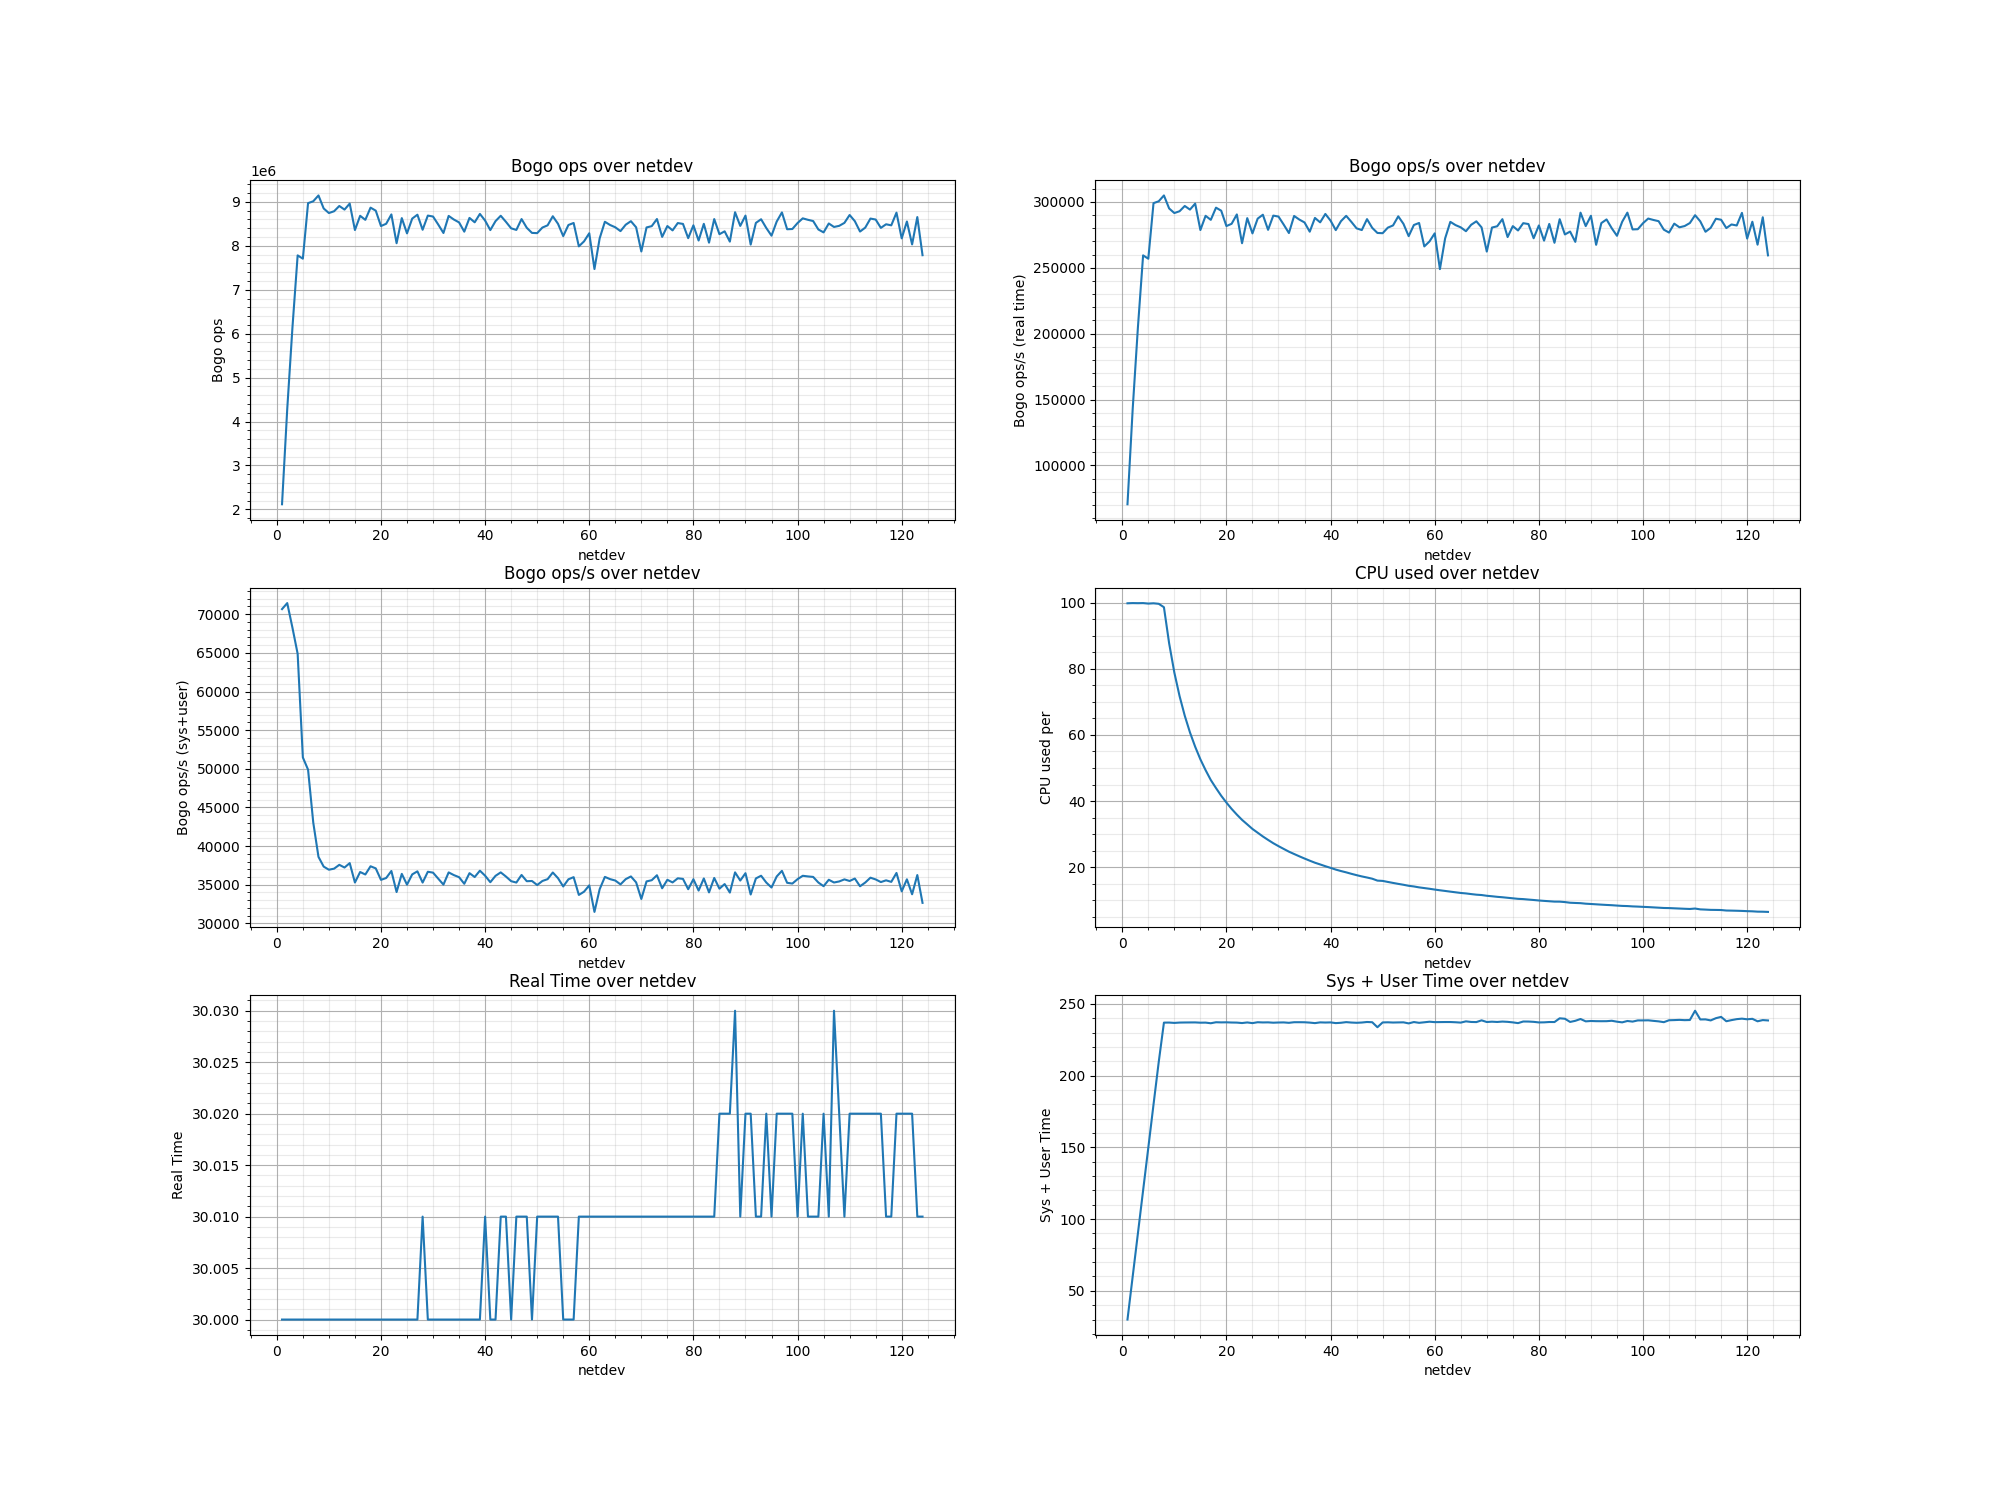
\includegraphics[width=\textwidth]{./network/image/netdev-bogops.png}
Максимум bogo ops достигается при 8.
Командой \textit{strace} мы можем посмотреть на команды, которые отправляет netdev сетевым интерфейсам:\\
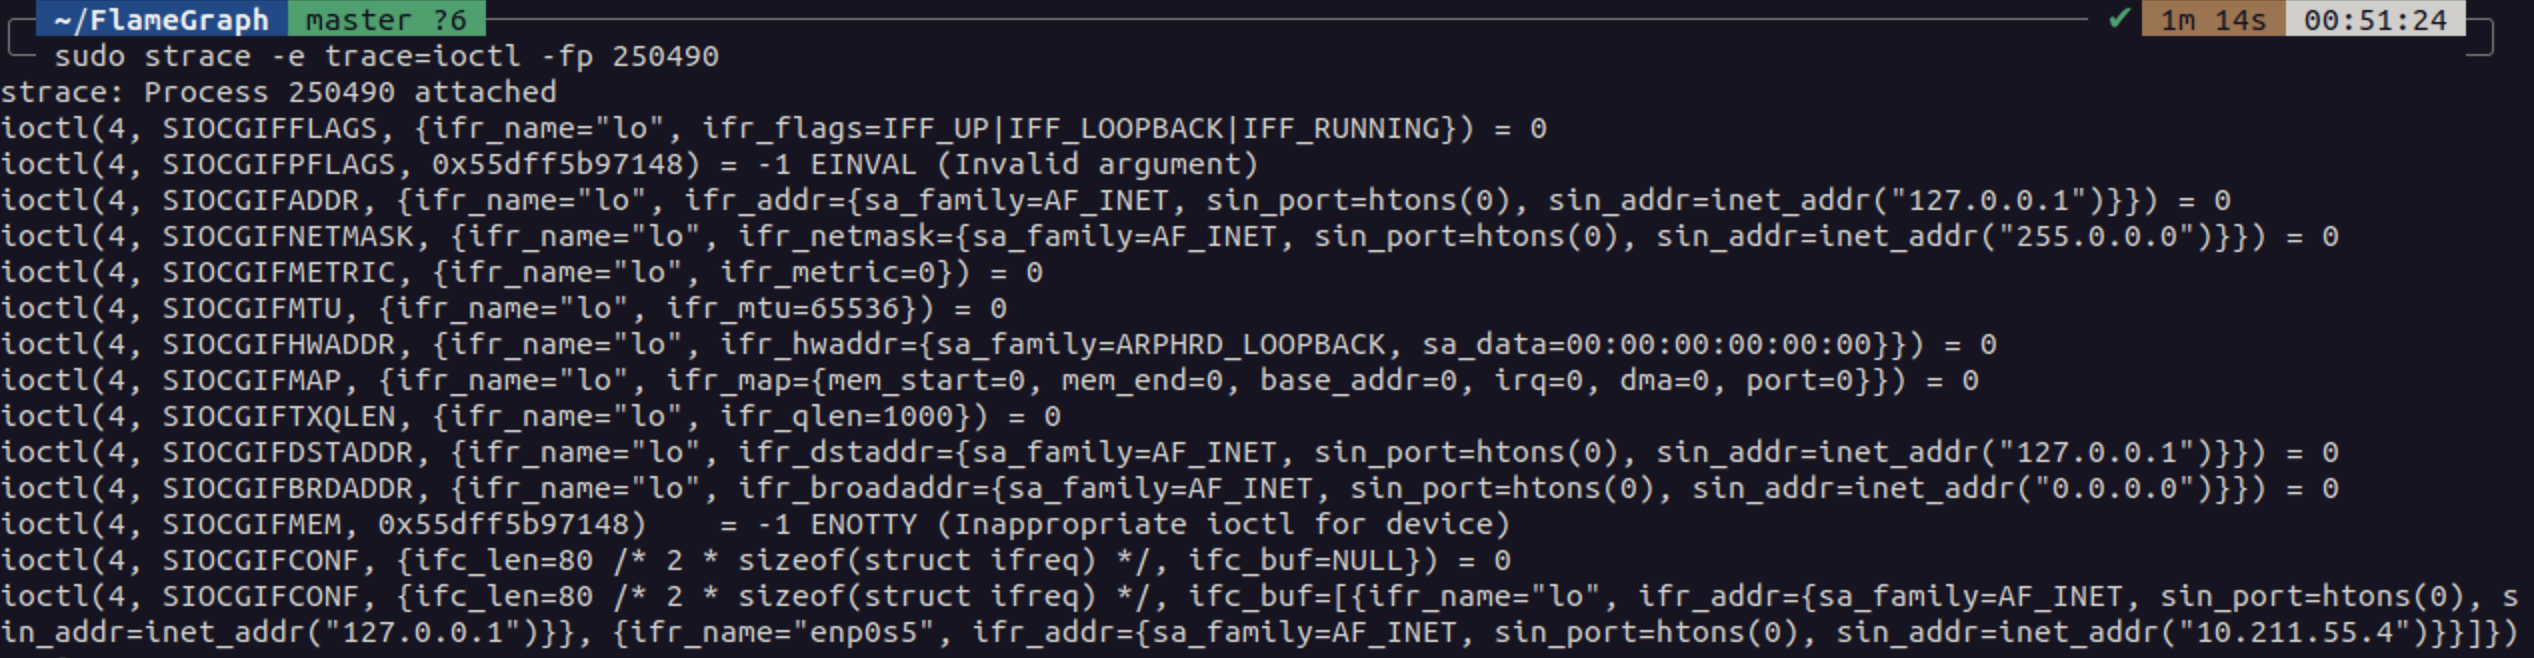
\includegraphics[width=\textwidth]{./network/image/netdev-strace.png}

